
% SEP 2012 Group 13
% Software Design Document (SDD)
%
\documentclass[11pt, a4paper]{report}
\usepackage{graphicx}
\usepackage{fullpage}
\usepackage{url}
\pagestyle{headings}

%%% page parameters
\headsep = 25pt
\begin{document}
\oddsidemargin -0.5 cm
\evensidemargin -0.5 cm
\textwidth 15 cm
\topmargin -1.2 cm
\textheight 25 cm
\begin{center}

\includegraphics[scale=1.5]{./UniLogo}\\[1cm]    
\textbf{\Huge \bfseries Software Design Document}\\[1.5cm]
\textbf{\huge for}\\[0.5cm]


% Title
\textbf{ \huge Archaeology Robot }\\[0.3cm]
\textbf{ \huge Group 13 }\\[2cm]


\begin{tabular}{ |c | p{2cm} |}
	\hline
Yufeng Bai 1600095 & \\[.5cm] \hline
Dawei Geng 1219181 & \\[.5cm] \hline
Jun Chen 1206265 & \\[.5cm] \hline
Quang Khoi Nguyen 1187070  & \\[.5cm] \hline
Shikai Li 1214223 & \\[.5cm] \hline
Yunyao Yao 1203525 & \\[.5cm] \hline
Yatong Zhou 1204471 & \\[.5cm] \hline
\end{tabular}


\vfill

% Bottom of the page
Version 1.31 \\ [0.2cm]
{\large \today}

\end{center}
\tableofcontents



% Version History %

% IMPORTANT %
% Whenever you make a change to this document you MUST put an entry in below
% Must conform to firstName lastName &  date & discription \\ \hline


\clearpage
\section*{Revision History}
\begin{tabular}{| l | l | l | l | }
\hline
Name				&	Date        	&	Reason For Changes                  	  	&	Version     	\\ \hline
Dawei Geng			&	03 Sep 2012     &	Template			                    	&	0.1 	    	\\ \hline
Yufeng Bai			&	06 Sep 2012	&	Chapter 7							&	0.2		\\ \hline
Yufeng Bai			&	06 Sep 2012	&	Chapter 8							&	0.3		\\ \hline
Yufeng Bai			&	06 Sep 2012	&	Chapter 9							&	0.4		\\ \hline
Yufeng Bai			&	07 Sep 2012	&	Fix the layout						&	0.5		\\ \hline
Jun Chen    		&  	08 Sep 2012 	&	Chapter 1                  		  	&	0.6     	\\ \hline
Jun Chen   		&	08 Sep 2012 	&	Chapter 2                 	  			&	0.7     	\\ \hline
Yufeng Bai			&	09 Sep 2012	&	Fix the error						&	0.8		\\ \hline
Khoi Nguyen 		&	10 Sep 2012     &	Chapter 4,5             				&	0.9     	\\ \hline
Jun Chen			&	11 Sep 2012	&	Chapter 3.1,3.2                	  		&	1.0    	\\\hline
Yufeng Bai			&	12 Sep 2012	&	Fix grammar and spelling errors			&	1.1		\\ \hline
Yatong Zhou      	&	12 Sep 2012     &	Chapter 6 and error fixing				&	1.2     	\\ \hline
%Name      		&	Date        	&	Reason For Changes                  	  	&	Version     	\\ \hline
%Name      		&	Date        	&	Reason For Changes                  	  	&	Version     	\\ \hline
%Name      		&	Date        	&	Reason For Changes                  	  	&	Version     	\\ \hline
%Name      		&	Date        	&	Reason For Changes                  	  	&	Version     	\\ \hline
%Name      		&	Date        	&	Reason For Changes                  	  	&	Version     	\\ \hline
%Name      		&	Date        	&	Reason For Changes                  	  	&	Version     	\\ \hline
%





\end{tabular}
\clearpage

% Introduction %

\chapter{Introduction}% (fold)
\label{cha:I}
%Provide an overview of the SDD and a description of the scope of the system to be developed.%


\section{Purpose and Scope}
\subsection{Purpose}
The purpose of making this Software Design Document (SDD) is to give the details of the design of the archaeology robot and its system, which is designed by our group (group 13). In this document, we will give an overall description of architectural design, system organisation and critical modules of the system. This document describes some general ideas of how do we design the system and how do we implement requirements into the system. This document will be given to the team members so that they can construct the system based on the requirements. Also this document will be used as a reference for further developments.
%Define the purpose of this document, specify intended readership of the docu- ment.%


\subsection{Scope}
This Software Design Document (SDD) is to give details  of overall design of archaeology robot. It will contain nine parts : Introduction which will give an overall description of the design, System Overview which will show the design of the system, System Architecture and Components Design, Architectural Description which also includes alternatives and rationale, Data Design, Human Interface Design, Resource Estimates and Definitions, Acronyms and Abbreviations.
%Identify the context of the system; explain what the proposed system does (and what does not, if necessary); describe the relevant benefits, objectives and goals. The description should be consistent with your SRS.%


\section{References}
This Software Design Document (SDD) references these files below:
\begin{enumerate}

  \item Software Requirements Document (SRS) : this document demonstrate all the requirements for this project.

  \item Software Project Management Plan (SPMP) : this document shows the details of how do we manage our project.

  \item UML files : the class diagram show how do we design and implement our system.

\end{enumerate}
%Provide a complete list of all documents that you referenced in SDD.%


\section{Overview}
This Software Design Document will be organised in a way that describe System, Architectural Design, GUI Design and Resource Estimates logically. In the beginning of the document, it will give an introduction of this document (Purpose and Scope) and System Overview. After that, the document will give some high level architectural design of the whole system, which include System Architecture and Components Design, Architectural Description. Then the document will move to the Data Design, which also includes Design Details. After the Data Design, it will also shows the design of Human Interface and Resource Estimates. Lastly, there are some Definitions, Acronyms and Abbreviations at the end of the document. This document will follow the developing stages.
%Overview the content of the document; explain how the SDD is organized.%

\section{Constraints}
The follow restrictions, limitations, and constraints will affect the design and implementation of the system:
\begin{itemize}
  \item The robot should be set up correctly before testing.
  \item The robot can not be damaged.
  \item The robot can not walk out of map.
  \item The robot can not push the wall and colliding is not permitted.
  \item The map should be set up correctly before testing
  \item The map is in fixed size (less than A1)
  \item There are some no-go zone on the map.
  \item The system must has save and load function.
  \item An acceptable latency is 300ms.
  \item There are some hidden wall in the map.
\end{itemize}
%Briefly describe any restrictions, limitations, and constraints that affect the design and implementation of the system.%


% chapter Introduction (end)
\pagebreak


\chapter{System Overview}% (fold)
\label{cha:SO}
The main goal of the system is to let the robot can be used for survey an archaeological site containing the remnants of an ancient city on the premise that the robot can not be damaged.
\par\vspace{\baselineskip}
\par\vspace{\baselineskip}
 Firstly, the system of the robot will use light sensor, touch sensor and ultrasonic sensor to locate some objects on the map, which include:
\begin{itemize}
  \item walls
  \item hidden walls
  \item obstacles on the surface
\end{itemize}
Secondly, the robot which is used to survey an archaeological site is programmed by leJOS software. With this software we can design the functionalities of the robot correctly, so that it can detect every object on the map on the premise that the robot is not damaged. When the robot detect somethings, the system should deal with it by using a proper way which is described in the Software Requirements Document (SRS).
\par\vspace{\baselineskip}
\par\vspace{\baselineskip}
Thirdly, the operating software of the robot will have a nice graphic user interface (GUI) which contains:
\begin{itemize}
  \item Control panel
  \item Map area
  \item robot information
  \item battery usage
  \item mode
  \item etc..
\end{itemize}
Lastly, the database of this project shall contain XML map files to store and update the survey map, the map shows :
\begin{itemize}
  \item the whole map
  \item No-go zone
  \item detected walls
  \item detected hidden wall
  \item detected obstacles
  \item unexplored zone
  \item explored zone
  \item the boundary of the map
  \item initial point
\end{itemize}

In conclusion, the whole system of this project contains four parts:
\begin{itemize}
  \item Client System which is installed in the robot for implementing its functionalities.
  \item User(Host) System which is used to control the robot and do things the clients want.
  \item GUI System is used to give a graphic user interface to the User System so that it is easier to be used.
  \item Database System which will store the survey result into a XML map.
\end{itemize}
With these four parts the system will work properly and do the task based on the requirements.

%Briefly introduce the system context and design.%


% chapter System Overview (end)
\pagebreak


\chapter{System Architecture and Components Design}% (fold)
\label{cha:SACD}
%In this section, you should cover the following content, in several subsections.%


\section{Architectural Description}
The archaeology robot system we make will has 4 major parts that work together effectively and achieve the goal. These four parts are Client System, Host System, Graphic User Interface System and Database System.
\paragraph{Client System: }The Client System is installed into the archaeology robot. Basically the Client System will be implemented all basic functionalities of the robot, like movement function. Also it is required to respond to commands which are sent from the Host System. Moreover the Client System should also include functionalities that can make the robot move automatically.
\newline
\paragraph{Host System: }The main purpose of the Host System is to control the movement of the robot so that it can survey the map manually. To meet this goal, all commands that control the robot will be implemented into the Host System, which include movement, stop, slow down, etc. Also it will be able to update the database according to the commands user make. The Host System will be able to stop the Client System, which means  the Host System is high priority. The Host System will also include function to change between manual mode and automatic mode.
\newline
\paragraph{GUI System: }The purpose of the GUI System is to combine most of the useful functions in a graphic way which is convenient for user to control the robot. With GUI System user can keep track of the position of the robot. Also the GUI System will show all information about the map and robot which means user can send commands to the Client System via GUI System. Moreover the GUI System can save(load) files to(from) the Database System.
\newline
\paragraph{Database System}The Database System is used to store the survey result of the archaeology robot. The Database System stores results by using XML files. The Database will implement a map for storing result.

%Describe the architectural design of the whole system. Typically, you should include a block diagram showing the major subsystems and their interconnec- tions.%

\section{Component Decomposition Description}
\subsection{Client} The Client will use Bluetooth to connect to the Host. It allows commands that are sent from the Host to be received and convert them into the commands that the Client can use. After executing the commands it will return feedbacks to the Host for updating Database.
\subsection{Host} The Host is the most important part in the system. It will be able to send commands to the Client (robot), also it can receive feedback from the Client (robot). Moreover, the Host shows every detail and change to the user by the GUI and it can update the database by sending commands. The components of Host include:
\paragraph{ManualController} is the main part of the Host. It is used to control the robot to perform any actions safely and precisely. Also it need to deal with the feedbacks that sent from the Client, which means it need to analyse them and then update the Database and show any changes on the GUI.
\paragraph{AutoController} will be used when the robot is in auto mode. It will disable most of all commands from the users (except Mode change command). The AutoController will determine the safe performances by analysing the current map via ultrasonic sensor. After analysing the Client will act automatically.
\subsection{GUI} The GUI will be implemented to the host. It will contain two components which include:
\paragraph{Main GUI} is the graphic interface for the host system which is used to show to the user. The main frame of it has many small components which act like functions, it includes the controlling of the robot, some icons, robot status, system status, save/load map and menu.
\paragraph{Map viewer} is a component of the GUI that shows the surveying map. It is used to display the location of the robot and draw the real map into it, which means the map viewer will display and draw everything the robot explored. After the survey, the map viewer will save the map into the database if it receive a save command which is sent by the Host.
\subsection{Database} The Database component is used to store the map after survey (survey value). The Database uses XML files to store the survey map. It allows the user to save XML files in it, also it allows the user to load any XML files which is stored in the Database. The Database only receive commands from the Host.
\paragraph{XML files} is used to store the 2D maps which are explored by the robot. Also some special zones will be stored into the map. The zones includes information of no-go zones, unexplored zone and explored zone. Zone will be represented as some blocks(pixels).
%A decomposition of the subsystems that summarizes the software components.%


\section{Detailed Components Design Description}
%Give the detailed design for each component. In particular, for each component, you need to provide:
%? Component Identifier: An identifier unique to this component.
%? Purpose: A reference (link) back to the requirement specification (SRS).
%? Function: What does this component do? Describe its functionality.
%? Subordinates: The components used by this component.
%? Dependencies: Constraints placed on this component by other compo- nents.
%? Interfaces: Control and data flow in and out of the component.
%? Data: Description of internal data if there is any.
\subsection{Interfaces}
\subsubsection{Client}
\begin{itemize}
\item Component Identifier: C-0
\item Purpose(function): to detail method declaration and what needs to implement
to control the movement of the robot such as moving, turning left, turning right, stop
\item Subordinates:client.BluetoothClient and client.RobotClient.
\item Dependencies: none
\item Interfaces: none
\item Data:The interface stores information related to the Client, %which
%includes command operation bits, definitions for boolean responses with byte values and
%masks to separate data from commands.
\end{itemize}

\subsubsection{Controller}
\begin{itemize}
\item Component Identifier: C-1
\item Purpose(Function): to detail method declaration and what needs to implement
for calls made by host.ui.UserInterface classes to the controller class
\item Subordinates:host.Driver
\item Dependencies: none
\item Interfaces: none
\item Data:none
\end{itemize}

% %Controller
% %ID C-1 Type Interface Class host
% %Purpose Abstracting the method declaration and implementation for calls made by
% %host.ui.UserInterface classes to the Controller classes.
% %%Function Provides a structure for method calls to any implementation. shall define the
% %parameters to be given and returned by methods that use this inerface
% %Subordinates host.MasterController
% %Dependancies none.
% %Interfaces none.
% %Data none.

\subsubsection{Database}
\begin{itemize}
\item Component Identifier: C-2
\item Purpose (Function) : to detail method declaration and
what needs to implement to create map, load map and save map
\item Subordinates:database.XMLDatabase
\item Dependencies: none
\item Interfaces: none
\item Data:none
\end{itemize}


% Database
% ID C-2 Type Interface Class host.database
% Purpose Abstracting the method declaration and implementation for the database module
% for outside calls.
% Function Provides a structure for method calls to any implementation of a class implementing
% the Database interface.
% Subordinates database.XMLDatabase
% Dependancies none.
% Interfaces none.
% Data none.
% Map
\subsubsection{Map}
\begin{itemize}
\item Component Identifier:  C-3
\item Purpose(Function): to detail method declaration and what needs to implement
to get and set the state of the map as well as get the position of the robot
\item Subordinates:database.ArrayMap
\item Dependencies: none
\item Interfaces: none
\item Data: none
\end{itemize}
% Map
% ID C-3 Type Interface Class host.database
% Purpose Abstracting the method declaration and implementation of any map functionality
% to be used by a class implementing the Database interface.
% Function Provides a structure for method calls to any implementation.
% Subordinates database.ArrayMap
% Dependancies none.
% Interfaces none.
% Data none.
\subsubsection{User Interface}
\begin{itemize}
\item Component Identifier: C-4
\item Purpose(Function): to detail method declaration and what needs to implement
 to allow the user of changing the map and the database, tog notifying of found walls
\item Subordinates:host.ui.GUI
\item Dependencies: none
\item Interfaces: none
\item Data:none
\end{itemize}
% UserInterface
% ID C-4 Type Interface Class host.ui
% Purpose Abstracting the method declaration and implementation for the GUI module.
% Function Provides a structure for method calls to any implementation. Calls that will
% be implemented by a GUI class are defined here.
% Subordinates host.ui.GUI
% Dependancies none.
% Interfaces none.
% Data none.
% 19
\subsection{Class Files}
\subsubsection{Driver}
\begin{itemize}
\item Component Identifier: C-5
\item Purpose: initialising the system and coordinating the operations,
which include communication between the host and the client, path finding,
loading and saving map.
\paragraph{SRS requirement:} touches almost all of the requirements
\item Function:The class creates host.database.XMLDatabase, a host.MasterController,
a client.Client and host.ui.GUI object.The Driver creates client.BluetoothClient object to communicate to the client. It also saves and load a map
 into a XML file. It makes call to the AutoController for the next move.
\item Subordinates:host.Controller,host.database.Database, host.ui.UserInterface and
 client.Client, host.AutoController, client.BluetoothClient,
host.database.XMLDatabase, host.database.Map and host.ui.GUI
\item Dependencies: host.Controller,host.database.XMLDatabase, host.ui.GUI,
 client.SimulationClient and client.BluetoothClient
\item Interfaces: Controller, Database, User Interface, Client
\item Data: storing the module objects and the flag variables to determine a simulation
or real connection; object detection parameters and threshold; minimum move and rotation distances
\end{itemize}
% ID C-5 Type Class Class
% Purpose This class runs the initial setup of the entire system. Defining the interconnections
% between the each component.
% Function This class creates a host.database.XMLDatabase, a host.MasterController,
% a client.Client and host.ui.GUI object. It will pass the host.database.Database
% and client.Client classes nothing, the host.MasterController the already created
% client.Client and host.database.Database objects. It will create the GUI using
% the host.MasterController object and client.Client before adding the GUI to the
% host.MasterController object.This class also accepts an argument of either nothing,
% where it will setup the system for a real connection to the robot, or ?-s? to setup the
% system with a simulated client
% Subordinates host.Controller,host.database.Database, host.ui.UserInterface &
% client.Client.
% Dependancies host.MasterController,host.database.XMLDatabase, host.ui.GUI,
% client.SimulationClient & client.BluetoothClient.
% Interfaces host.Controller,host.database.Database, host.ui.UserInterface &
% client.Client.
% Data Holds the four module objects as data and the flag variable to determine a simulation
% or real connection.

% \subsubsection{Master Controller}
% \begin{itemize}
% \item Component Identifier: C-1
% \item Purpose: to coordinate the operation of the entire system. The operations
% include commnunication between the host and the client, path finding,
% loading and saving map.
% \paragraph{SRS requirement:} R0001: Manual Robot Movement, R0003: Automatic Robot Movement,
% R0004: Automatic Exploration, R0005:Avoiding danger under automatic mode,
% R0009: Robot Mode Change, R0011: Load/Save XML
% \item Function: The Master Controller creates client.BluetoothClient object to communicate to the client. It also saves and load a map
%  into a XML file. The class makes call to the AutoController for the next move.
% \item Subordinates:host.AutoController, client.BluetoothClient, host.database.Point,
% host.database.XMLDatabase, host.database.Map and host.ui.GUI
% \item Dependencies: host.Controller
% \item Interfaces: Database, Map, Point
% \item Data:object detection parameters and threshold; minimum move and rotation distances
% \end{itemize}

% MasterController
% ID C-6 Type Class Class host
% Purpose This class will act as part of the interface between the GUI and the client. It
% will use a client.BluetoothClient object to communicate commands to the client. Each
% command should first have a series of checks, for safety purposes, before calling on the
% client.BluetoothClient object. It will also read and write to a database containing all
% relevant information that the GUI requires. This includes the ability to save and load
% a current minefield map into a saved XML file. The MasterController class will make
% calls to the AutomaticUser class to return the next logical move for automated control.
% SRS requirements U-3, U-4, U-5, U-6, U-7, U-8, S-0, S-1, S-2, S-3, N-2 & N-3.
% Function The MasterController class shall create Client, Database & GUI objects to
% interact with. It will pass the GUI a Database object from which to draw its data from and
% itself as a Host object from which it shall relay user commands. The MasterController
% object will have no main method and only function on methods called by the GUI object.
% Subordinates host.AutomaticUser, client.BluetoothClient, host.database.Point,
% host.database.XMLDatabase, host.database.Map & host.ui.GUI
% Dependancies host.Controller
% Interfaces host.database.Database, host.database.Map, host.database.Point,
% host.ui.UserInterface & client.Client.
% Data sweep Offsets, object detection parameters and thresholds, mine detection parameters
% and thresholds & minimum move and rotation distances.
% Host

\subsubsection{AutoController}
\begin{itemize}
\item Component Identifier: C-6
\item Purpose: to autonomously exploring the map safely
\paragraph{SRS requirement:} R0004: Automatic Exploration, R0005: Avoiding danger
\item Function: The method will take a Map file and then determine the robot?s current location, bearing and then possible moves.
It always check if a move is safe before  executing
\item Subordinates:host.database.Map and client.Client.
\item Dependencies: host.Controller
\item Interfaces: Controller
\item Data: the position of the robot relative to the walls
\end{itemize}
% AutomaticUser
% ID C-7 Type Class Class host
% Purpose This class shall perform all functionality to determine a safe autonomously
% moving robot. It shall ensure SRS requirements U-4, N-2 & N-3.
% Function This calls will take a Map object and use it to determine the robot?s current
% location, bearing and then possible moves. The class will follow the state diagram in
% section 5.11.2 of this document. Whenever a manual movement is going to be executed
% host.MasterController will first implement one of AutoMaticUser?s safety check functions
% to check a safe move is to be executed.
% Subordinates host.database.Map & client.Client.
% Dependancies host.Controller
% Interfaces host.Controller
% Data Movement safety check offset co-ordinates relative to the front left wheel.
\subsubsection{BlueToothClient}
\begin{itemize}
\item Component Identifier: C-7
\item Purpose: to act as an intermediary between the host and client.
\paragraph{SRS requirement:}R0001: Manual Robot Movement, R0004: Automatic Move Robot,
R0005: Automatic robot exploration, R0011:Load and Save XML Files
\item Function: When a command parameter is parsed into the method, the command is sent to
client.BluetoothHost.
\item Subordinates:client.BluetoothHost and host.MasterController
\item Dependencies: client.Client.
\item Interfaces: Controller, Client
\item Data: none
\end{itemize}
% BluetoothClient
% ID C-8 Type Class Class client
% Purpose To transmit a signal from the host machine to the client and have a reply signal
% to return to the host machine. SRS requirements N-4 and U-10
% Function This Java class shall create an object to be implemented within a BasicHost
% object to implement robot movement, a sweep method and interrogate the robot for data
% readings.. This class shall follow the client interface and be able to communicate with
% a client.BluetoothHost object via a Bluetooth link. it shall transmit a Bluetooth signal
% from the host machine to the client. When a method is called it will receive a parameter.
% It shall then call the send command, passing both the operator command value, declared
% within the Client interface, and the parameter which the original method call was given.
% The send command will then handle the transmission and receiving of data between the
% BluetoothClient and client.BluetoothHost.
% Subordinates client.BluetoothHost & host.MasterController
% Dependancies client.Client.
% Interfaces host.Controller, client.Client
% Data none.

\subsubsection{BluetoothHost}
\begin{itemize}
\item Component Identifier: C-8
\item Purpose: to act as an intermediary between the host and client.
\paragraph{SRS requirement:} R0001: Manual Robot Movement, R0004: Automatic Move Robot,
R0005: Automatic robot exploration, R0011:Load and Save XML Files
\item Function: opening a I/O stream to get input from client.BluetoothClient.
Client.BluetoothHost remains in an infinite loop while waiting for a command.
\item Subordinates:client.RobotClient
\item Dependencies: none
\item Interfaces: Client
\item Data:none
\end{itemize}


% BluetoothHost
% ID C-9 Type Class Class client
% Purpose To receive command trasmissions from the a client.BluetoothClient object.
% SRS requirements N-4 and U-10.
% Function This class opens a Bluetooth I/O stream to receive input from a
% client.BluetoothClient object over the communications interface. client.BluetoothHost
% will remain within an infinite while loop trying to receive a command from the I/O
% stream.
% Subordinates client.RobotClient.
% Dependancies none.
% Interfaces client.Client
% Data none.

\subsubsection{Robot}
\begin{itemize}
\item Component Identifier: C-9
\item Purpose: to move the robot and to record the detected features
\paragraph{SRS requirement:}R0001: Manual Robot Movement, R0004: Automatic Move Robot,
R0005: Automatic robot exploration, R0011:Load and Save XML Files
\item Function: The robot client receives command from a client.BluetoothHost and then perform
accodingly. If it detects any features of the area, it will return data to client.BluetoothHost.
\item Subordinates: none
\item Dependencies: client.BluetoothHost
\item Interfaces:  Client
\item Data: the position of the robot, the speed and angles that the light sensor should rotate
, the collected data
\end{itemize}


% RobotClient
% ID C-10 Type Class Class client
% Purpose To physically move the robot using a client.Client interface. SRS requirements
% U-5, U-7 & S-0.
% Function This class will receive method calls from a client.BluetoothHost object. Its
% methods will instruct the Mindstorm robot to respond to commands given by the host
% machine and return data requested by the host machine.
% Subordinates none.
% Dependancies client.BluetoothHost
% Interfaces client.Client
% Data Variables to tune the dimensions of the robot, speed & angles which the lightsensor
% arm must rotate to collect data at the correct points.
\subsubsection{XML Database}
\begin{itemize}
\item Component Identifier: C-10
\item Purpose: to be a map database for a host machine. Maps can be loaded and saved by the
class.
\paragraph{SRS requirement:} R0011: Load and Save XML File
\item Function: initializing a  database.Map object and allows the creation of a map through
the database.Map class. The class has method to get the state of the map such as pixel data and
different zones. It is able to set and get the position of the client on the map. The current state
of map can be saved to an XML file. A unfinished or finished map can also be loaded into XMLDatabase.
\item Subordinates:host.database.xmlParser and host.database.ArrayMap
\item Dependencies: host.database.DataBase and host.database.Map
\item Interfaces: Database and Controller
\item Data: none
\end{itemize}

% XMLDatabase
% ID C-12 Type Class Class host.database
% Purpose Act as an XML map database for a host machine. Maps may be loaded and
% saved through this class. SRS requirements U-3, S-2 & S-3
% Function instantiates a database.Map object and allows the creation of a map through
% the database.Map class. Has methods to retrieve zone and pixel data through the
% database.Zone class. Is able to set the Client?s position on the map with a bearing and
% return the data through a getRobotPosition method. The current state of a map shall be
% saved to an XML file at a given file-path when requested. A previous map may then be
% loaded into the XMLDatase when requested.
% Subordinates host.database.xmlParser & host.database.ArrayMap.
% Dependancies host.database.DataBase & host.database.Map
% Interfaces host.database.DataBase & host.Controller
% Data
\subsubsection{Zone}
\begin{itemize}
\item Component Identifier: C-11
\item Purpose: To store the state of each grid zone into 4 pixels (sub-grids)
\paragraph{SRS requirement:} R0011: Load and Save XML File
\item Function: initialising the 4 pixels as unexplored. The class can set and get the state
of a pixel, which is represent as a pre-defined integer.
\item Subordinates: host.database.Map
\item Dependencies: host.database.Map
\item Interfaces: Map
\item Data:variables storing the states of the zone's four areas.
\end{itemize}

% Zone
% ID C-14 Type Class Class host.database
% Purpose To store the state of each grid zone into 4 pixels (sub-grids) that the
% database.XMLDatbase object shall use to gather data on a database.Map?s current state.
% SRS requirement U-3, S-2, S-3.
% Function This class shall initialise the 4 pixels within the database.Zone object as unexplored,
% the unexplored static final variable shall be stored within the database.Database
% interface, and shall be changed though the database.Database Object with a setPixelState
% method. Accompanying the setPixelState method will be a getPixelState method which
% shall return the current state of a pixel as an integer value. State?s are defined within the
% database.Database interface.
% Subordinates host.database.Map
% Dependancies host.database.Map
% Interfaces host.database.Map
% Data The Zone class contains four variables for the Zone?s four quadrants, each is set to
% a state defined in the host.database.Map interface
\subsubsection{Map}
\begin{itemize}
\item Component Identifier: C-12
\item Purpose: to create a map storing states of small grids in a two dimensional arrays
\paragraph{SRS requirement:} R0011: Load and Save XML File
\item Function:initialising the map to be the size of a grid, which is two by two. As the robot
 explores the map, it calls setBoarder method to increase the size of the map. The state of each
 pixel can be set and accessed through the setPixel and getPixel methods

\item Subordinates:host.database.Point and host.database.Zone.
\item Dependencies: host.database.Map
\item Interfaces: Map and Database
\item Data: a two-dimensional array storing Zone objects
\end{itemize}

% ArrayMap
% ID C-15 Type Class Class host.database
% Purpose To store the state of each grid as a database.Zone object within a 2d array of
% Zone objects. SRS requirement U-3, S-2 & S-3.
% Function The map shall be created with a height and width of the rectangular grid space.
% A boarder for the minefield may be created within this rectangular grid space with a
% setBoarder method. The state of each pixel of each zone is accessible through setPixel
% and getPixel methods which shall call the methods within database.Zone to return pixel
% states
% Subordinates host.database.Point & host.database.Zone.
% Dependancies host.database.Map
% Interfaces host.database.Map & host.database.Database
% Data this class contains a 2d-array of Zone objects that are stored with an associated
% state variable defined in the host.database.Map class.
\subsubsection{MapPanel}
\begin{itemize}
\item Component Identifier: C-13
\item Purpose: to display the graphical representation of the map
\paragraph{SRS requirement:} R0007: Map Representation
\item Function: The map is displayed using information from the database. The map shows
the position of the robot and its traveled distance
\item Subordinates: host.database.Map and host.database.Database.
\item Dependencies: host.ui.UserInterface
\item Interfaces: Map and Database
\item Data: position of the robot and how far the robot has travelled.
\end{itemize}
%
% mapPanel
% ID C-17 Type Class Class host.ui
% Purpose To display the graphical representations of the map
% Function The map will be displayed using information stored in the map database and
% set out in a grid
% Subordinates host.database.Map & host.database.Database.
% Dependancies host.ui.UserInterface.
% Interfaces host.ui.UserInterface.
% Data This class contains current GUI position data. How far the user has zoomed in,
% how far he has moved centre of the map in both x and y co-ordinates.
% 27

\subsubsection{GUI}
\begin{itemize}
\item Component Identifier: C-14
\item Purpose: an interface in the host machine to control and keep track of the robot
\paragraph{SRS requirement:} R0008: Robot representation,R0009: Robot mode change,
R0007: Map representation
\item Function: manually controlling the robot, entering the autonomous exploring mode, updating
the battery and signal status
\item Subordinates: host.ui.MapPanel, host.ui.MasterController and host.ui.XMLDatabase.
\item Dependencies: host.ui.UserInterface and host.Controller
\item Interfaces: UserInterface and Controller
\item Data: predefined representation of functionalities on the screen, the current state of the robot.
\end{itemize}

% GUI
% ID C-18 Type Class Class host.ui
% Purpose To provide the user with an interface to communicate with the robot and display
% the information of the minefield
% Function Confirms the location of the mine, updates the current display, gets information
% of the battery status, as well as the signal strength. It also connects to the database
% and the host.
% Subordinates host.ui.MapPanel, host.ui.MasterController & host.ui.XMLDatabase.
% Dependancies host.ui.UserInterface & host.Controller
% Interfaces host.ui.UserInterface & host.Controller
% Data This class must have a list of predefined colour variations it will use to show objects
% on the screen. It must also keep track of what mode it is currently in to determine what
% will show on screen.
\section{Architectural Alternatives}
%Discuss briefly other architectures that were considered if any.%
The other alternative design which is considered is letting the robot do the exploration without
waiting command from the host. The idea is shelved because the robot's resource is not capable
of performing the algorithm.

%Need more details

% Other architectures are considered in the design of the system. One of them we considered is
% to indicate the logically finding a path on the robot itself. Then the robot accesses into the bordered
% areas of the map and detect the objects(mines, obstacles or beacons)in order to perform safe
% and successful mission. This design is scraped on the basis that the robot does not have enough
% memory or processing capacity to store the data and execute the commands efficiently.In another
% design, bordered areas will be represented by a bitmap rather than polygonal shapes. This will
% have simplified the logic involved with clipping and merging zones together as well as navigating
% through the map. However this is inconvenient to save the current map into an XML format file
% and will require converting between polygonal shapes and bitmap formats which is complex. This
% design has a limit on using a bitmap which means a very large map will not be able to represent
% the details or require a large amount of memory.

\section{Design Rationale}
%Discuss the rationale on selecting the architecture described in 3.1, including the critical issues and tradeoffs that were considered.%
The design of the system is layer architecture. The model is chosen for its support of separation
and independence. The development is spread across teams with each team being responsible
for a different part. The use of interface allows smooth integration without risk of
 incompatible method calls. If there is change in the interface, only the adjacent layer is affected
 so change is localised.

% chapter System Architecture and Components Design (end)
\pagebreak


\chapter{Data Design}% (fold)
\label{cha:DD1}
%You should cover database description and data structures in this section.%

\section{Database Description}
%Describe briefly the database(s) that is part of the system.%
The map is represented in XML format. It is created when the robot starts to explore.The map updates every time when the robot explores an area, detects
a wall or a border of the survey area. The information which is stored in the array is translated
and saved into XML. The XML file can be loaded as well. The detailed functionalities are
as follow:

\paragraph{Creating a map}

The map is initialised to be a size of a grid, which is two by two.
The size of the map is stored as digital number and the coordinates of the border are stored in an
array list.

\paragraph{Recording the features of the area}

\begin{itemize}
  \item  Clear Area: containing no features and is considered to be safe. The status and coordinate
   is saved if the area is explored.
\item	Wall Area: containing walls.The status and coordinate is saved if the area is explored.
\item  No-go-zone area: the robot is not permitted to enter the area. The status and coordinate is
entered by the operator.
\end{itemize}

\paragraph{Recording the position of the robot}

The coordinates of current position are stored in an array list and are flagged as visited.

\paragraph{Saving}

The map which is explored so far can be saved.

\paragraph{Loading}

The previous map can be loaded,

% The representation of database of the minefield in the host side is represented in XML format. It
% is created when the map on the host side is displayed. It is updated every time when the robot
% explorers a new area, detects a mine, an obstacle or finds a beacons in the minefield. All these
% status are translated into XML and saved in the XML file which can be reloaded for further use.
% The database includes following contents:


\section{Data Structures}
%Give the detailed design of the database, i.e., entities and their relationships. You can use either ER model or UML for this purpose.%
The underlying data structure of the map database is a two dimensional array. Each element
is the zone (grid)'s information, which is indexed by its coordinatting in the map. Each zone(grid)
consisted of the information of its 4 sub-grids, which is stored in a two-by-two array


% chapter Data Design (end)
\pagebreak

\chapter{Design Details}% (fold)
\label{cha:DD2}
%You shall describe your design by using the following diagrams to reflect all the major requirements that you documented in the SRS.%


\section{Class Diagrams}
%Describe all class diagrams that are considered in the system. Give the details (e.g., attributes, operations) associated with the class.%

\begin{figure}[h]
  \centering
    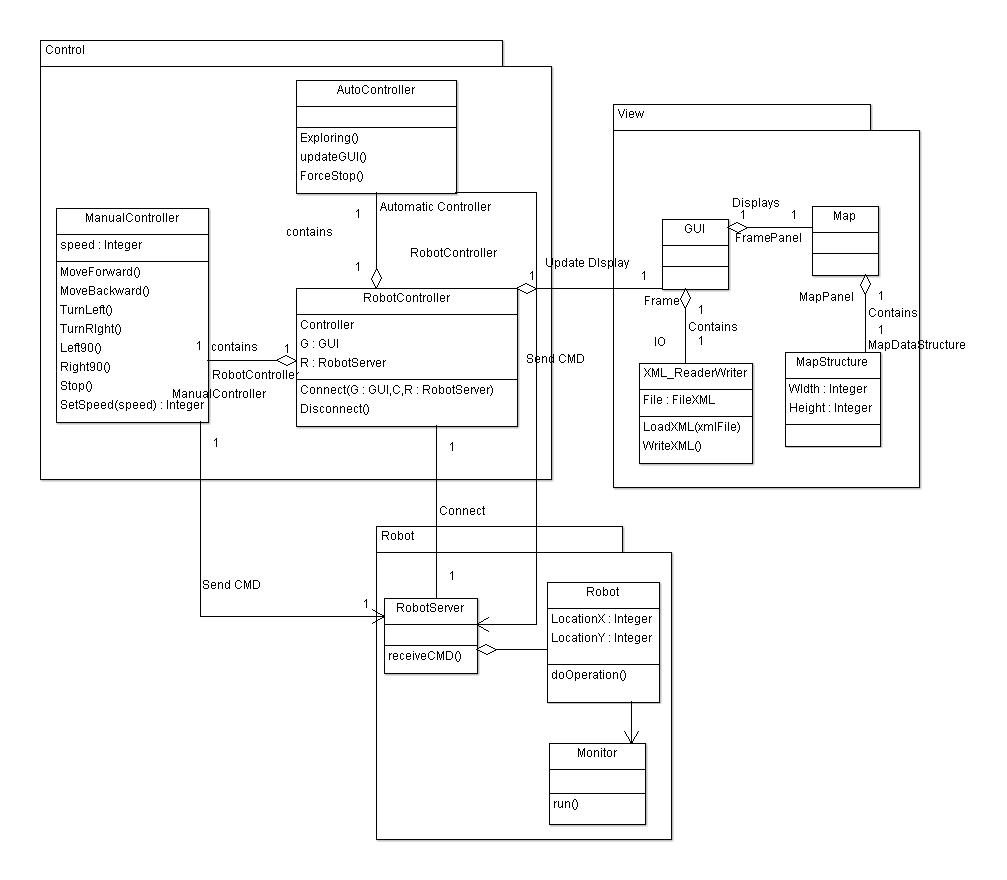
\includegraphics[width=16cm]{SEP_13_Class_Diagram.png}
  \caption{Class Diagram}
\end{figure}
The diagram above shows the package and class structures of the entire project. The class model follows the classic MVC design pattern. Model is the controller part of the project, which controls the robot. GUI is the view part, displays the map in the run-time. Model is the robot itself mechanism, which is able to be accepted the command from the controller.
\newpage



\section{State Diagrams}
%Present the state diagrams of objects involved.%
\begin{figure}[h]
  \centering
    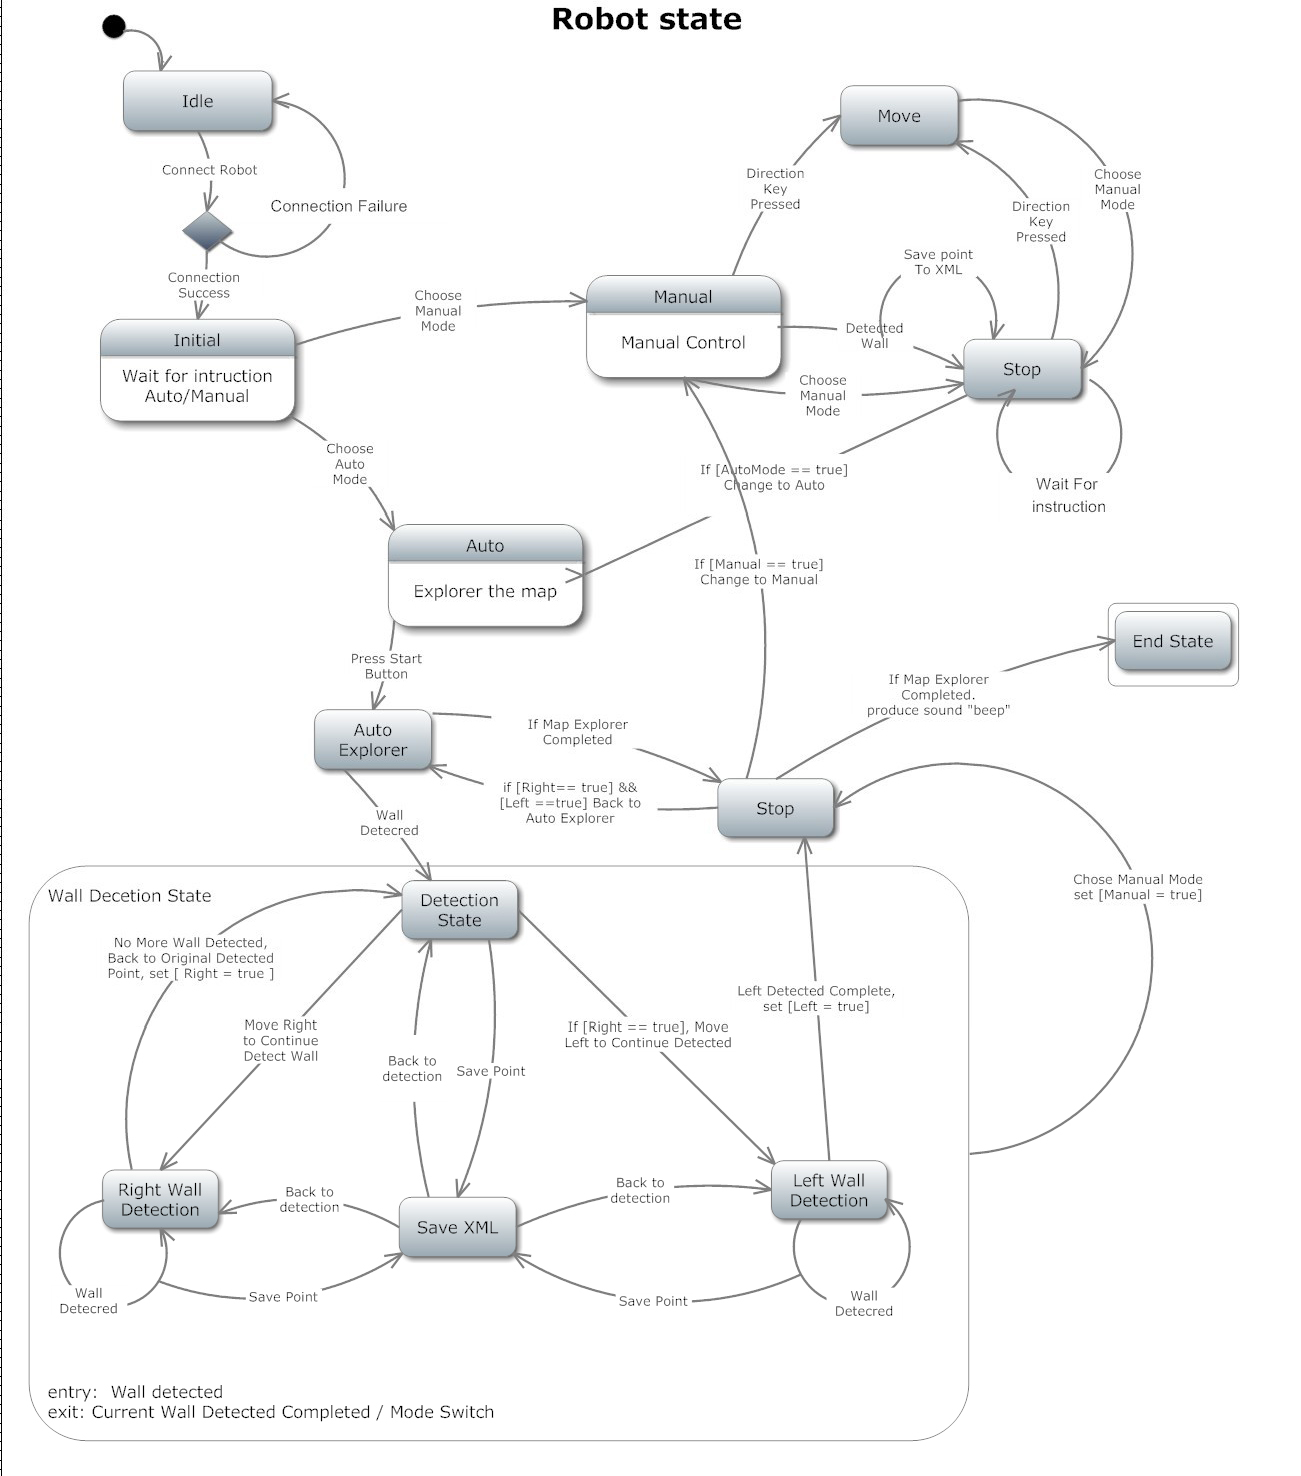
\includegraphics[width=16cm]{SEP_13_RobotStateDiagram.jpg}
  \caption{State Diagram}
\end{figure}
The state diagram above shows the all possible status of the robot. The robot started with initial state, after connecting, it jumps to "Idle" state, which means doing nothing but waiting for the commands from the host. After initial the map and establish connection. It wait operator to chose control mode. It transfers to either manual or auto control state to explore the unmapped areas. When transfer to auto mode(whatever in start or in the middle), robot will checks whether the map is fully explored. If yes, it reaches the end state. If not, the robot will do more exploration follow searching algorithms, if any wall is detected in the process, robot will record current location and start wall detection state, it will keep check the wall on left side until on more wall is found, and then check right side. After detected the wall, robot will come back to auto exploration mode. When transfer to Manual mode state, the robot can be control by operator, but for safety reason, if any wall is detected or go into no go zone in manual control, the robot will still pose its movement in until get next instruction that is safe to move. User can switch mode, and terminates exploring at any time.
\newpage


\section{Use Case Diagrams}
%Present the state diagrams of objects involved.%
\begin{figure}[h]
  \centering
    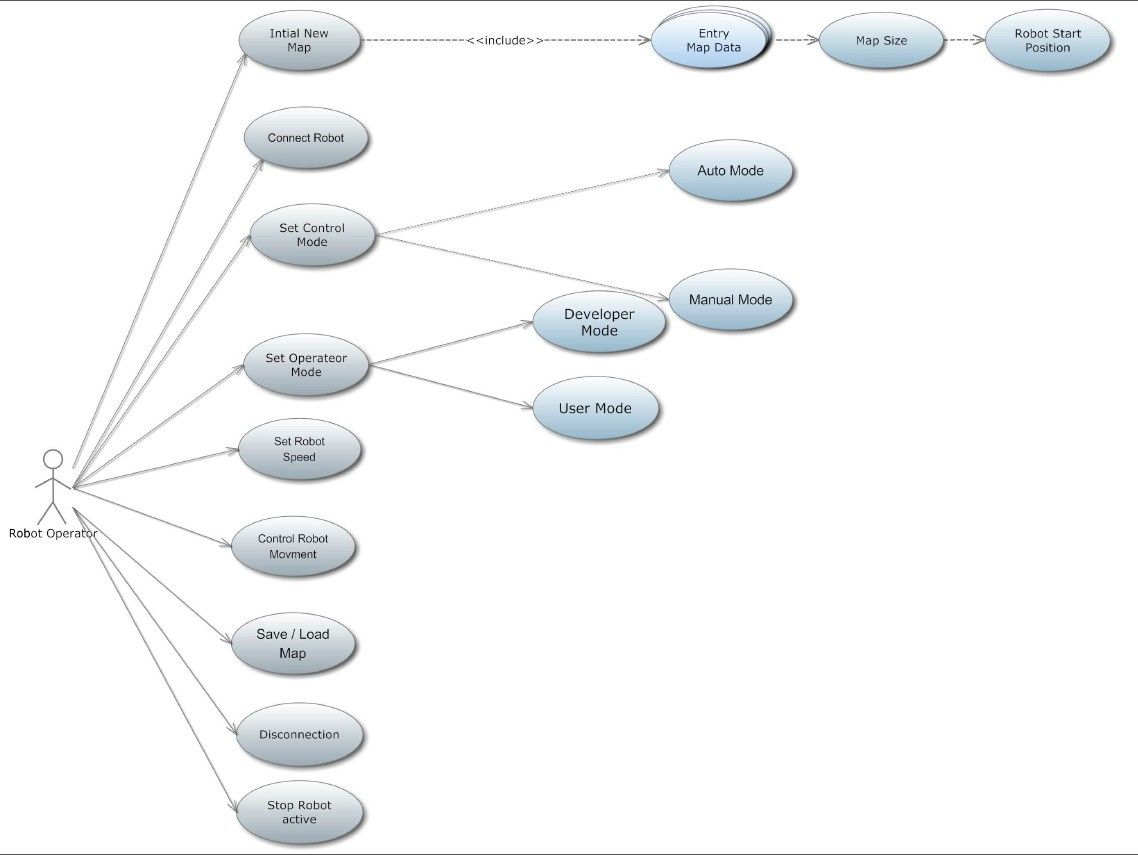
\includegraphics[width=16cm]{SEP_13_UseCase.jpg}
  \caption{Use Case Diagram}
\end{figure}
The use case diagram above shows all the cases that user can operate on the graphic user interface. Start with initial map, this allow user to set initial value of map like map height, weight and start coordinate. Also a serial of instruction to to set up robot. That include establish robot connection, set operator mode (User/Developer), set control mode(Auto/Manual) and set robot movement speed. After robot set up, user can control robot through the control panel to explore the map. In addition user can save map or load map in the process. User also can chose disconnect with the robot or terminate this exploration at any time.
\newpage


\section{Interaction Diagrams}
%Present the interactions of objects involved.%
%Note: all the diagrams shall be numbered and link to the requirements in%
%the SRS; UML notations should be strictly followed.%
\begin{figure}[h]
  \centering
    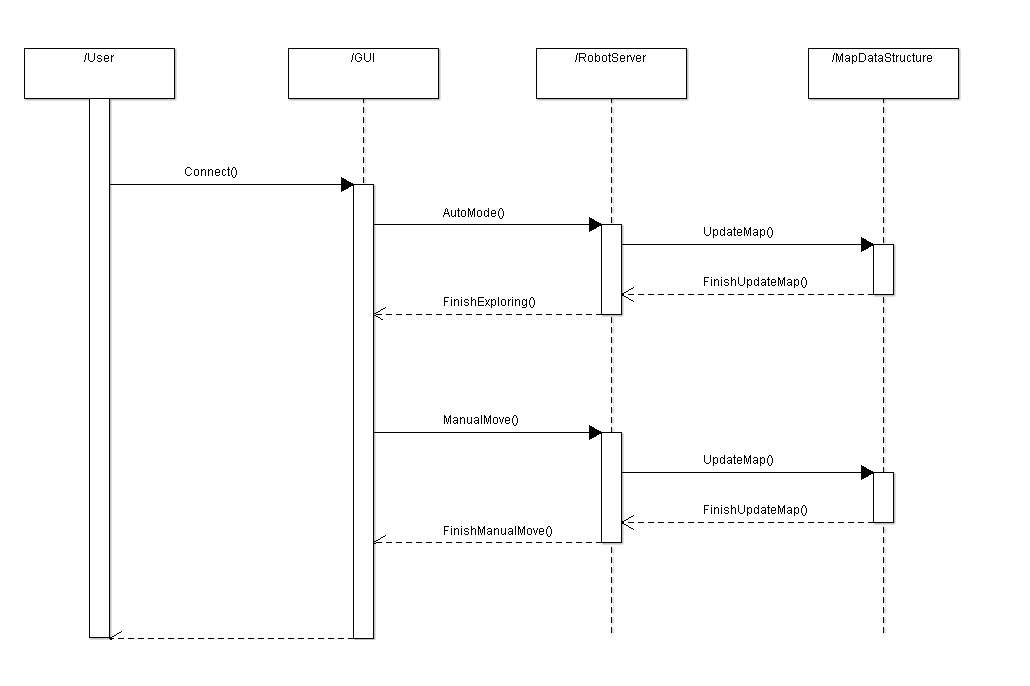
\includegraphics[width=16cm]{SEP_13_Sequence_Diagram.png}
  \caption{Interaction Diagram}
\end{figure}
The above diagram demonstrates how control is passed during the simple operation of the user manually moving the robot forward.
\\The GUI calls the hosts move function, which will do the required safeguard checks and then forward it onto the client, who will return the distance moved.
\\Afterwards the host will update the map data structure, so when the GUI updates the robot's new position and map display.

% chapter Design Details (end)
\pagebreak


\chapter{Human Interface Design}% (fold)
\label{cha:HID}

\section{Overview of the User Interface}
%Describe briefly the general functionalities of the system from end users? per- spective.%
The Graphical User Interface is used to communicate with the robot. The GUI is connected with robot, the client is able to control the robot by GUI. When the robot finishes its task, the client is allowed to switch off and disconnect with robot. In addition, the GUI demonstrates the status of the robot. The status includes the speed, the power and the location of the robot. The GUI also shows the obstacles, the "no-go" zone and hidden walls, which is able to be checked on the map window.\\

The GUI is able to demonstrate the follow functions for users:
\begin{itemize}
\item Save map to a XML file
\item Load map from a XML file
\item Change the control mode
\item Demonstrate the Bluetooth and Battery status
\item Control the moving direction of the robot(i.e. forward, backward, rotating)
\item Demonstrate the Icon of the map
\item Demonstrate the Log Information
\item Change the speed of the robot
\item Demonstrate the coordinate of the robot
\end{itemize}
The GUI is displayed below:
\pagebreak
\begin{center}
 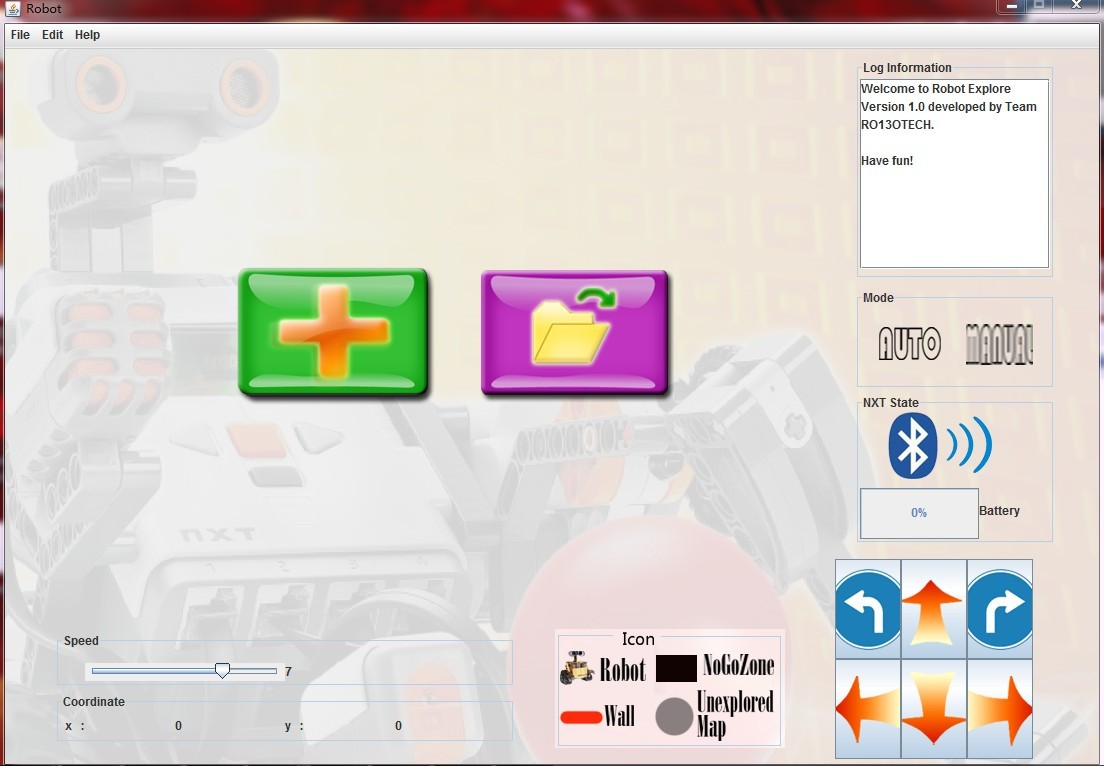
\includegraphics[width=11.20cm]{GUI.jpg}
\end{center}
\begin{center}
\textbf {Figure 11: GUI} \\[0.3cm]
\end{center}
\begin{center}
 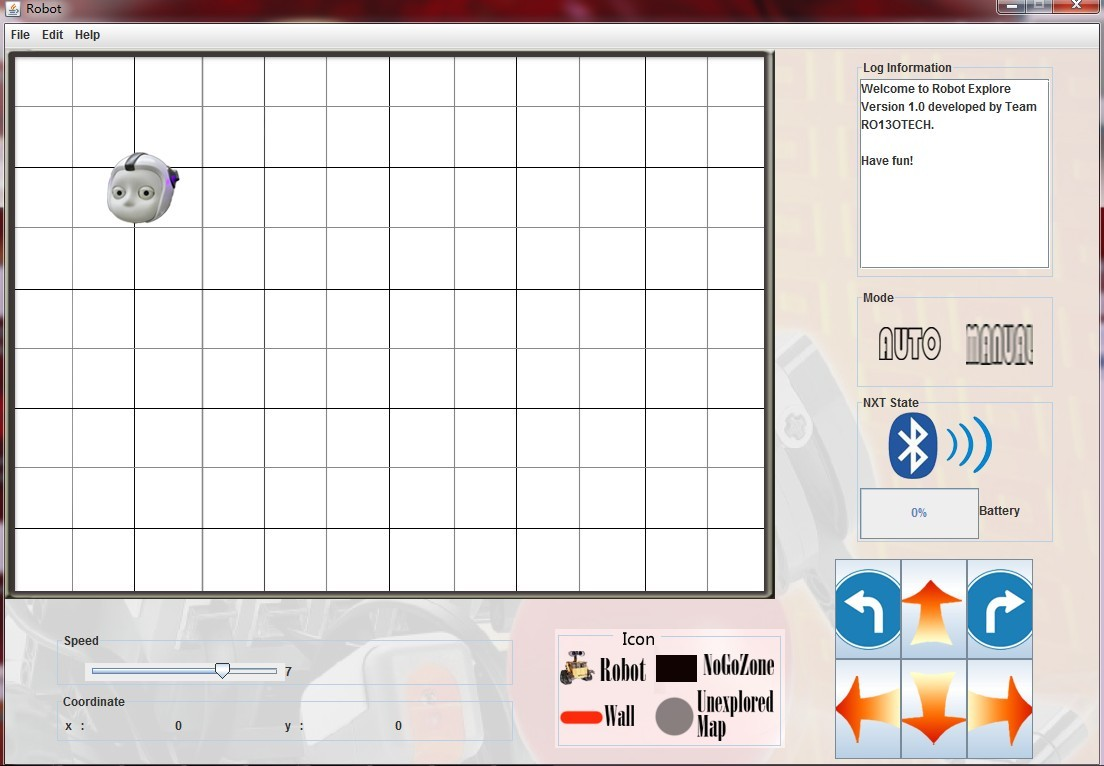
\includegraphics[width=11.20cm]{GUI2.jpg}
\end{center}
\begin{center}
\textbf {Figure 12: GUI WITH MAP} \\[0.3cm]
\end{center}
\section{Detailed Design of the User Interface}
\subsection{Save map}
The GUI includes a icon which is used to save the map from a XML file. When the client presses the File menu and choose the save option, there is a window jumping out, the client is able to choose the file where the client want to save.
\begin{center}
 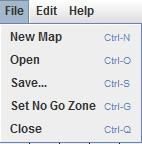
\includegraphics[width=9.20cm]{save}
\end{center}
\begin{center}
\textbf {Figure 13: SAVE MAP} \\[0.3cm]
\end{center}
\subsection{Load map}
The GUI includes a icon which is used to load the map from a XML file. When the client presses that icon, there is a window jumping out, the client is able to choose the map from there.
\begin{center}
 
\includegraphics[width=9.20cm]{load}
\end{center}
\begin{center}
\textbf {Figure 14: LOAD MAP} \\[0.3cm]
\end{center}
\subsection{Change the control mode}
The client is allowed to change the control mode by pressing the mode button. When the client presses the Auto mode button, there is a widget jumping out. Then if the client presses "yes", the robot changes to the Auto mode. The client is allowed to do the same operation to change to the Manual mode.  The Log information display which mode it is currently.
\begin{center}
 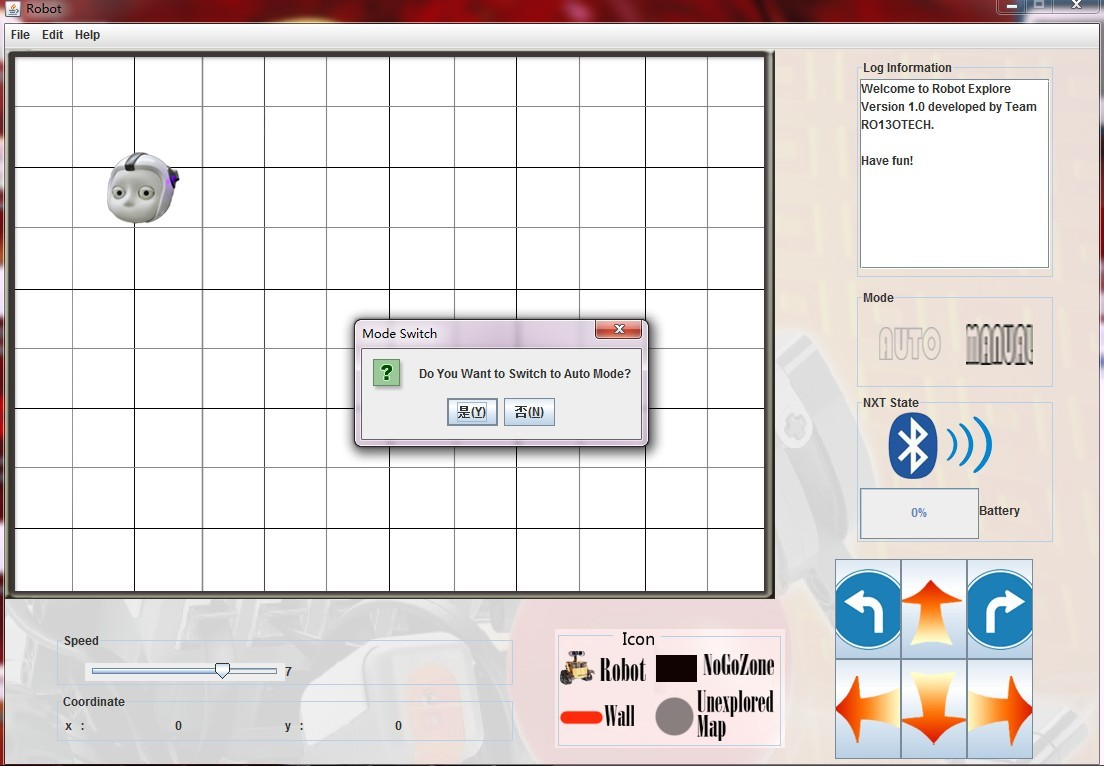
\includegraphics[width=11.20cm]{changemode.jpg}
\end{center}
\begin{center}
\textbf {Figure 15: Change Mode} \\[0.3cm]
\end{center}
\begin{center}
 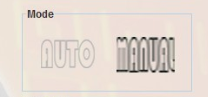
\includegraphics[width=11.20cm]{changemode2}
\end{center}
\begin{center}
\textbf {Figure 16: Change Mode icon} \\[0.3cm]
\end{center}
\subsection{Demonstrate the Bluetooth and battery status}
The Bluetooth and battery status are displayed on the GUI, if the bluetooth loses the connection, the log information board will demonstrate the lose information. The power of the battery is displayed by the percentage number and the colour of the battery bar will change along with the battery level.
 \begin{center}
 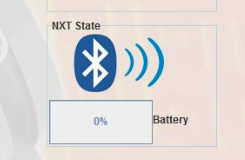
\includegraphics[width=11.20cm]{bluetooth_battery}
\end{center}
\begin{center}
\textbf {Figure 17: Bluetooth and battery demonstration } \\[0.3cm]
\end{center}
\subsection{Control the moving direction of the robot}
The robot is able to be controlled by GUI when the robot is changed to the Manual mode. The client is allowed to press the arrows to move the robot. The robot is able to move forward, backward and rotate(include rotate 90 angles and rotate 360 angles). The moving direction controlling only can be used in Manual mode.
 \begin{center}
 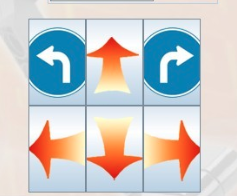
\includegraphics[width=11.20cm]{direction}
\end{center}
\begin{center}
\textbf {Figure 18: Moving control} \\[0.3cm]
\end{center}
\subsection{Demonstrate the icon of the map}
The robot and map information are required to be displayed on the GUI. It is necessary to use different icons to demonstrate the different map information.
  \begin{center}
 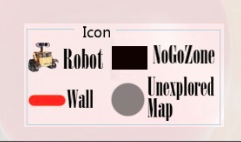
\includegraphics[width=11.20cm]{icon}
\end{center}
\begin{center}
\textbf {Figure 19: Icon of the map} \\[0.3cm]
\end{center}
\subsection{Demonstrate information of the GUI on the log information board}
The Log Information board displays the information of the GUI. For example, the Log Information board demonstrates the version and the developers of the robot. If the client changes the control mode, the board displays which mode it is now. The board also is required to indicate the connection information.
  \begin{center}
 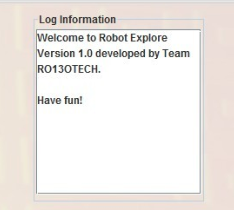
\includegraphics[width=11.20cm]{board}
\end{center}
\begin{center}
\textbf {Figure 20: The logging information} \\[0.3cm]
\end{center}
\subsection{Control the speed of the robot}
The GUI includes a speed bar and one specific number to control the speed of the robot. The client is allowed to change the speed of the robot by change the number of the bar. The larger number means the faster the robot is. If the number is zero, it means the robot stops immediately.
  \begin{center}
 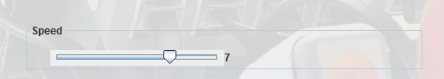
\includegraphics[width=11.20cm]{bar}
\end{center}
\begin{center}
\textbf {Figure 21: The speed controlling} \\[0.3cm]
\end{center}
\subsection{The location of the robot}
The GUI is required to display the specific location of the robot. The map is made up of a lot of grids. The location of the robot is able to display by coordinate, which is more accurate. When the robot moves, the coordinate will changes immediately.
   \begin{center}
 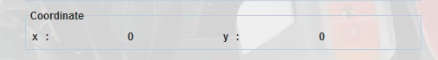
\includegraphics[width=11.20cm]{coordinate}
\end{center}
\begin{center}
\textbf {Figure 22: The coordinate of the robot} \\[0.3cm]
\end{center}


%You have to present your user interface design from the following perspectives:
%? Screen Images: screenshots showing the interface from end users? perspec- tive.
%? Screen Objects and Actions: discussion of screen objects and the actions associated with those objects.
%? Report Forms: a description of major reports provided by the system, if any.
%Note: all the interface designs have to link to the user requirements and functional requirements in the SRS; all the interface images shall be num- bered.


% chapter Interface Design (end)
\pagebreak




\chapter{Resource Estimates} % (fold)
\label{cha:RE}
%A summary of computer resource estimates required for operating the system.%
The resource of the project is estimated according to the Project Description and the client's requirements in every week's meeting. All hardware and software which are used in the project are demonstrated below.
\section{Hardware}
\subsection{Robot}
Name: NXT Robot includes all components of the robot\\
Function: The robot is used to search the map and find all the obstacles, hidden walls and "no-go" zone. All operations are required to finish by controlling the robot.
\subsection{Host}
Name: PC\\
Function: The PC is required to demonstrate the searching information of the robot. PC is also used to control the robot on Manual Mode. The programs are uploaded to the robot from the PC.
\subsection{Connection}
Name: Bluetooth and USB \\
Function: The Bluetooth and USB are all used to connect with the robot. The USB is limited by the length of the cable. The bluetooth is limited by the uploading speed. In this project, the USB is used to upload the program and the bluetooth is used to implement the manual control.
\section{Software}
\subsection{Operation Environment}
Name: Mac, Linux and Windows\\
Function: This project is not providing the working environment. Any system is able to develop the programs for the robot.
\subsection{Developing language}
Name: Java, latex\\
Function: The codes are allowed to write in java language, which is convenient to be read by any developers. The documents are required to write by Latex, then generating the pdf documents.
\subsection{Developing tool}
Name: Eclipse\\
Function: Eclipse is a better tool to make the program for this project. The Eclipse is used to write the operation commands for the robot and draw the GUI for this project.
\subsection{Robot Software}
Name: leJOS 0.9.1\\
 Function: The leJOS is used to control the robot and developing tool is required to support the leJOS 0.9.1.
 \subsection{Testing tool}
 Name: JUnit\\
 Function: The JUnit is used to debug the code.

% chapter Resource Estimates (end)
\pagebreak

\chapter{Definitions, Acronyms, and Abbreviations} % (fold)
\label{cha:DAA}
\section{Acronyms and Abbreviation}
\begin{center}
\begin{tabular}{|l|c|}
  \hline
  \textbf{Acronyms/Abbreviation} & \textbf{Description}\\
  \hline
  API		& Application Programmable Interface \\
  \hline
  BT		& Bluetooth \\
  \hline
  GUI		& Graphical User Interface \\
  \hline
  PC		& Personal Computer\\
  \hline
  SRS	& Software Requirements Specifications \\
  \hline
  SPMP 	& Software Project Management Plan \\
  \hline
  UML	& Unified Modelling Language\\
  \hline
  USB	& Universal Serial Bus\\
  \hline
  XML 	& eXtensible Markup Language \\
  \hline
\end{tabular} \\[0.3cm]
\textbf {Table 1: Acronyms/Abbreviations} \\[0.3cm]
\end{center}
%Provide definitions of all terms, acronyms, and abbreviations used in SDD.%
\section{Definitions}
\begin{enumerate}
\item API: A set of classes and interfaces which are used to make the program for the robot include PC API and lejos API.\\
\item BT: A device to implement the wireless connection.\\
\item GUI: A interface which is generated on the PC is used to send the commands to the robot.\\
\item PC: A device which is used to make the program for the robot and build the GUI.\\
\item UML: A modelling language is used to build the diagrams for the project.\\
\item USB: A device to implement the wired connection.\\
\item XML: The data structure is used to store the map information.\\
\end{enumerate}
% chapter Definitions, Acronyms, and Abbreviations (end)
\pagebreak
% Appendicies %
\newpage
\appendix

\pagebreak

\end{document}
